\documentclass[12pt]{article}
%%\usepackage[margin=1in]{geometry}
\usepackage{enumitem}
%\usepackage{forest}
%%para ver el directorio
\usepackage{dirtree}
\usepackage{fontawesome5}
\usepackage[utf8]{inputenc}
\usepackage{multicol}
\usepackage[T1]{fontenc}
\usepackage{fancyhdr}
\usepackage{titlesec}
\usepackage[breaklinks=true]{hyperref}
\usepackage[table]{xcolor}
\usepackage[customcolors]{hf-tikz}
\usepackage{listings}
\usepackage{graphicx} 
%%\usetikzlibrary{arrows,shapes,positioning,shadows,trees}
%%%%%%%%%%%%%%%%%%%%%%%%%%%%%%%%%%%%%%%%%
%colors
\definecolor{rositapastel}{RGB}{255, 135, 159}
\titleformat{\section}
            {\color{rositapastel}\normalfont\Large\bfseries}
            {\thesection}{1em}{}
\titleformat{\subsection}
            {\color{rositapastel}\normalfont\large\bfseries}
            {\thesubsection}{1em}{}

\titleformat{\subsubsection}
            {\color{rositapastel}\normalfont\normalsize\bfseries}
            {\thesubsubsection}{1em}{}
%%%%%%%%%%%%%%%%%%%%%%
% Mis comandos
\newcounter{recordatorioCounter}
\newcommand{\recordatorio}{%
  \stepcounter{recordatorioCounter}%% avanza el contador
  \textbf{\textcolor{rositapastel}{Recordatorio \therecordatorioCounter : }}
}
            
            
            
\lstdefinestyle{mystyle}{
  backgroundcolor=\color{rositapastel!23},   
  commentstyle=\color{codegreen},
  keywordstyle=\color{magenta},
  numberstyle=\tiny\color{codegray},
  stringstyle=\color{codepurple},
  basicstyle=\ttfamily\footnotesize,
  breakatwhitespace=false,         
  breaklines=true,                 
  captionpos=b,                    
  keepspaces=true,                 
  numbers=left,                   
  numbersep=5pt,                  
  showspaces=false,                
  showstringspaces=false,
  showtabs=false,                  
  tabsize=2
}

\lstset{style=mystyle}

% Icono Carpeta
\newcommand{\foldericon}{\faFolderOpen~}

\definecolor{foldercolor}{RGB}{255, 193, 7}
\definecolor{pdfcolor}{RGB}{220, 53, 69}
\definecolor{readmecolor}{RGB}{40, 167, 69}

\renewcommand{\foldericon}{\textcolor{foldercolor}{\faFolder}}
\newcommand{\pdficon}{\textcolor{pdfcolor}{\faFilePdf}}
\newcommand{\txticon}{\textcolor{txtcolor}{\faFileAlt}}
\newcommand{\zipicon}{\textcolor{gray}{\faFileArchive}}



% Set up fancy header/footer
\pagestyle{fancy}
\fancyhead[LO,L]{UNAM}
\fancyhead[RO,R]{\textit{\textsc{Proyecto}}}   
\fancyfoot[LO,L]{Facultad De Ciencias, 2027-I}
\fancyfoot[CO,C]{\thepage}
\fancyfoot[RO,R]{Modelado y Programación}
\renewcommand{\headrulewidth}{0.4pt}
\renewcommand{\footrulewidth}{0.4pt}
%%%%%%%%%%%%%%%%%%%%%%

\newdimen\digitwidth
\settowidth\digitwidth{0}
\def~{\hspace{\digitwidth}}

% Cambiar color de secciones
\titleformat{\section}
            {\color{rositapastel}\normalfont\Large\bfseries}
            {\thesection}{1em}{}

\titleformat{\subsection}
            {\color{rositapastel}\normalfont\large\bfseries}
            {\thesubsection}{1em}{}

\titleformat{\subsubsection}
            {\color{rositapastel}\normalfont\normalsize\bfseries}
            {\thesubsubsection}{1em}{}

% Cambiar color de ítems en listas numeradas
\setlist[enumerate]{label=\textcolor{rositapastel}{\arabic*.}, left=1.5em}
\setlist[itemize]{label=\textcolor{rositapastel}{\alph*}, left=1.5em}
\setlist[itemize]{label=\textcolor{rositapastel}{\textbullet}, left=1.5em}


\begin{document}
\begin{titlepage}
  \begin{center}

    \textsc{\Large\uppercase{Universidad Nacional Autónoma De México}}\\[0.4cm]	

    {\huge \Large \uppercase{Facultad de Ciencias, 2027-I} \\[0.4cm] }
    {\huge \Large \uppercase{Facultad de Ciencias} \\[1cm] }

    %%\includegraphics[scale=.2]{image.png}\\[0.6cm]


    %%% Título
    \rule{\linewidth}{0.4pt}\\[0.7em]
         { \color{rositapastel} \textsc{\Large Proyecto:}} \\[0.7em] 
         \textit{\Large Rolas}
         \\[0.1em] 
         \rule{\linewidth}{0.4pt}\\[2em]


         \color{black!80!black}{\large \uppercase{\textsc{ Profesor:}}}\\[0.25cm]

         \begin{tabular}{l}
           \large Canek Pelaez Valdez \\[0.4cm]
         \end{tabular}

         \large \uppercase{Ayudante de Teoría:}\\[0.2cm]
         \centering
         \begin{tabular}{l}

           \large Cynthia Lizbeth Sánchez Urbano \\[0.4cm]
         \end{tabular}

         \large \uppercase{Ayudante de Laboratorio:}\\[0.2cm]
         \centering
         \begin{tabular}{l}

           \large Miriam Torres Bucio\\[0.4cm]
         \end{tabular}

         \vfill

  \end{center}
\end{titlepage}


\section*{Introduccion}

Se debe crear una base de datos de canciones que se pueda editar, a traves de una interfaz gráfica, agregar canciones de archivos mp3 con etiqueta ID3v2.4.0 utilizando un minero y poder buscar en la base de datos creando un compilador que pueda pasar las instrucciones del usuario a busquedas en sql.

\section*{Analisis y diseño}

Como se explicó en la introducción, el proyecto se divide en dos partes, \textbf{Minero}, \textbf{Interfaz} y el minero debe poder funcionar de forma independiente, por lo que creé dos programas disttinros, llamados, evindentemente Minero e Interfaz.

\subsection*{Minero}
\subsubsection*{Analisis}
EL minero lo decidí hacer en c++, porque cuando investigué encontré la biblioteca de archivos, para poder leer directorios, ya que existe una función que permita hacerlo recursivamente muy fácil.
Primero, en mi main solamente creo mi objeto Minero y uso su método mina que de igual manera usa mi objeto lector, recorre directorios y que a su vez usa el objeto Filtro que es el que se encarga de validar la etiqueta ID3 v2.4.0 y el objeto basededatos es el que guarda los datos que contenga el archivo en la base de datos.

\subsubsection*{Diseño}
Hice 5 distintas clases, cada una con una función diferente:
\subsubsection*{Aplicación}
En Aplicación solamente se lee la ruta del directorio a minar a traves de la entrada estándar y se crea un Minero que minará el directorio y sus subdirectorios.

\subsubsection*{Minero}
Minero lo único que hace es usar un Lector para leer los directorios, realmente solo lo hice para que se llamara minero y no lector.

\subsubsection*{Lector}

El lector, que tiene un único método ``leeDirectorio(const string\& s)'', utiliza la biblioteca filesystem, que se usa para, con la ruta dada, acceder a los archivos y recursivamente, con ``recursive\_directory\_iterator'' se recorren los subdirectorios y de hecho por la facilidad de hacer esto es porque escogí c++ y, mientras se recorre cada archivo uso el método ejecuta de mi objeto Filtro para leer las etiquetas de los archivos que sean válidos.  

  \subsubsection*{Filtro}
  
  Filtro es el que lee las etiquetas ID3 v2.4.0 y agrega cada campo a la base de datos, además de imprimir si si son mp3 con esa etiqueta o si no tiene ningun dato que leer. el método más largo es el de PrintInformation() que realmente lo copié de el repositorio de la biblioteca que uso, pero e cambié unas cosas para poder agregar las imagenes donde quiero y asignar los valores de campoCancion.

  \subsubsection*{Base de Datos}
  Base de datos conecta a la base de datos que se tiene, además de agregar y eliminar en esta, tambien tiene una struct campoCancion que permite asignar los valores de la tabla rola con lo que se encuentre en las etiquetas.

    \newpage
  
\begin{figure}[htbp]
    \centering
    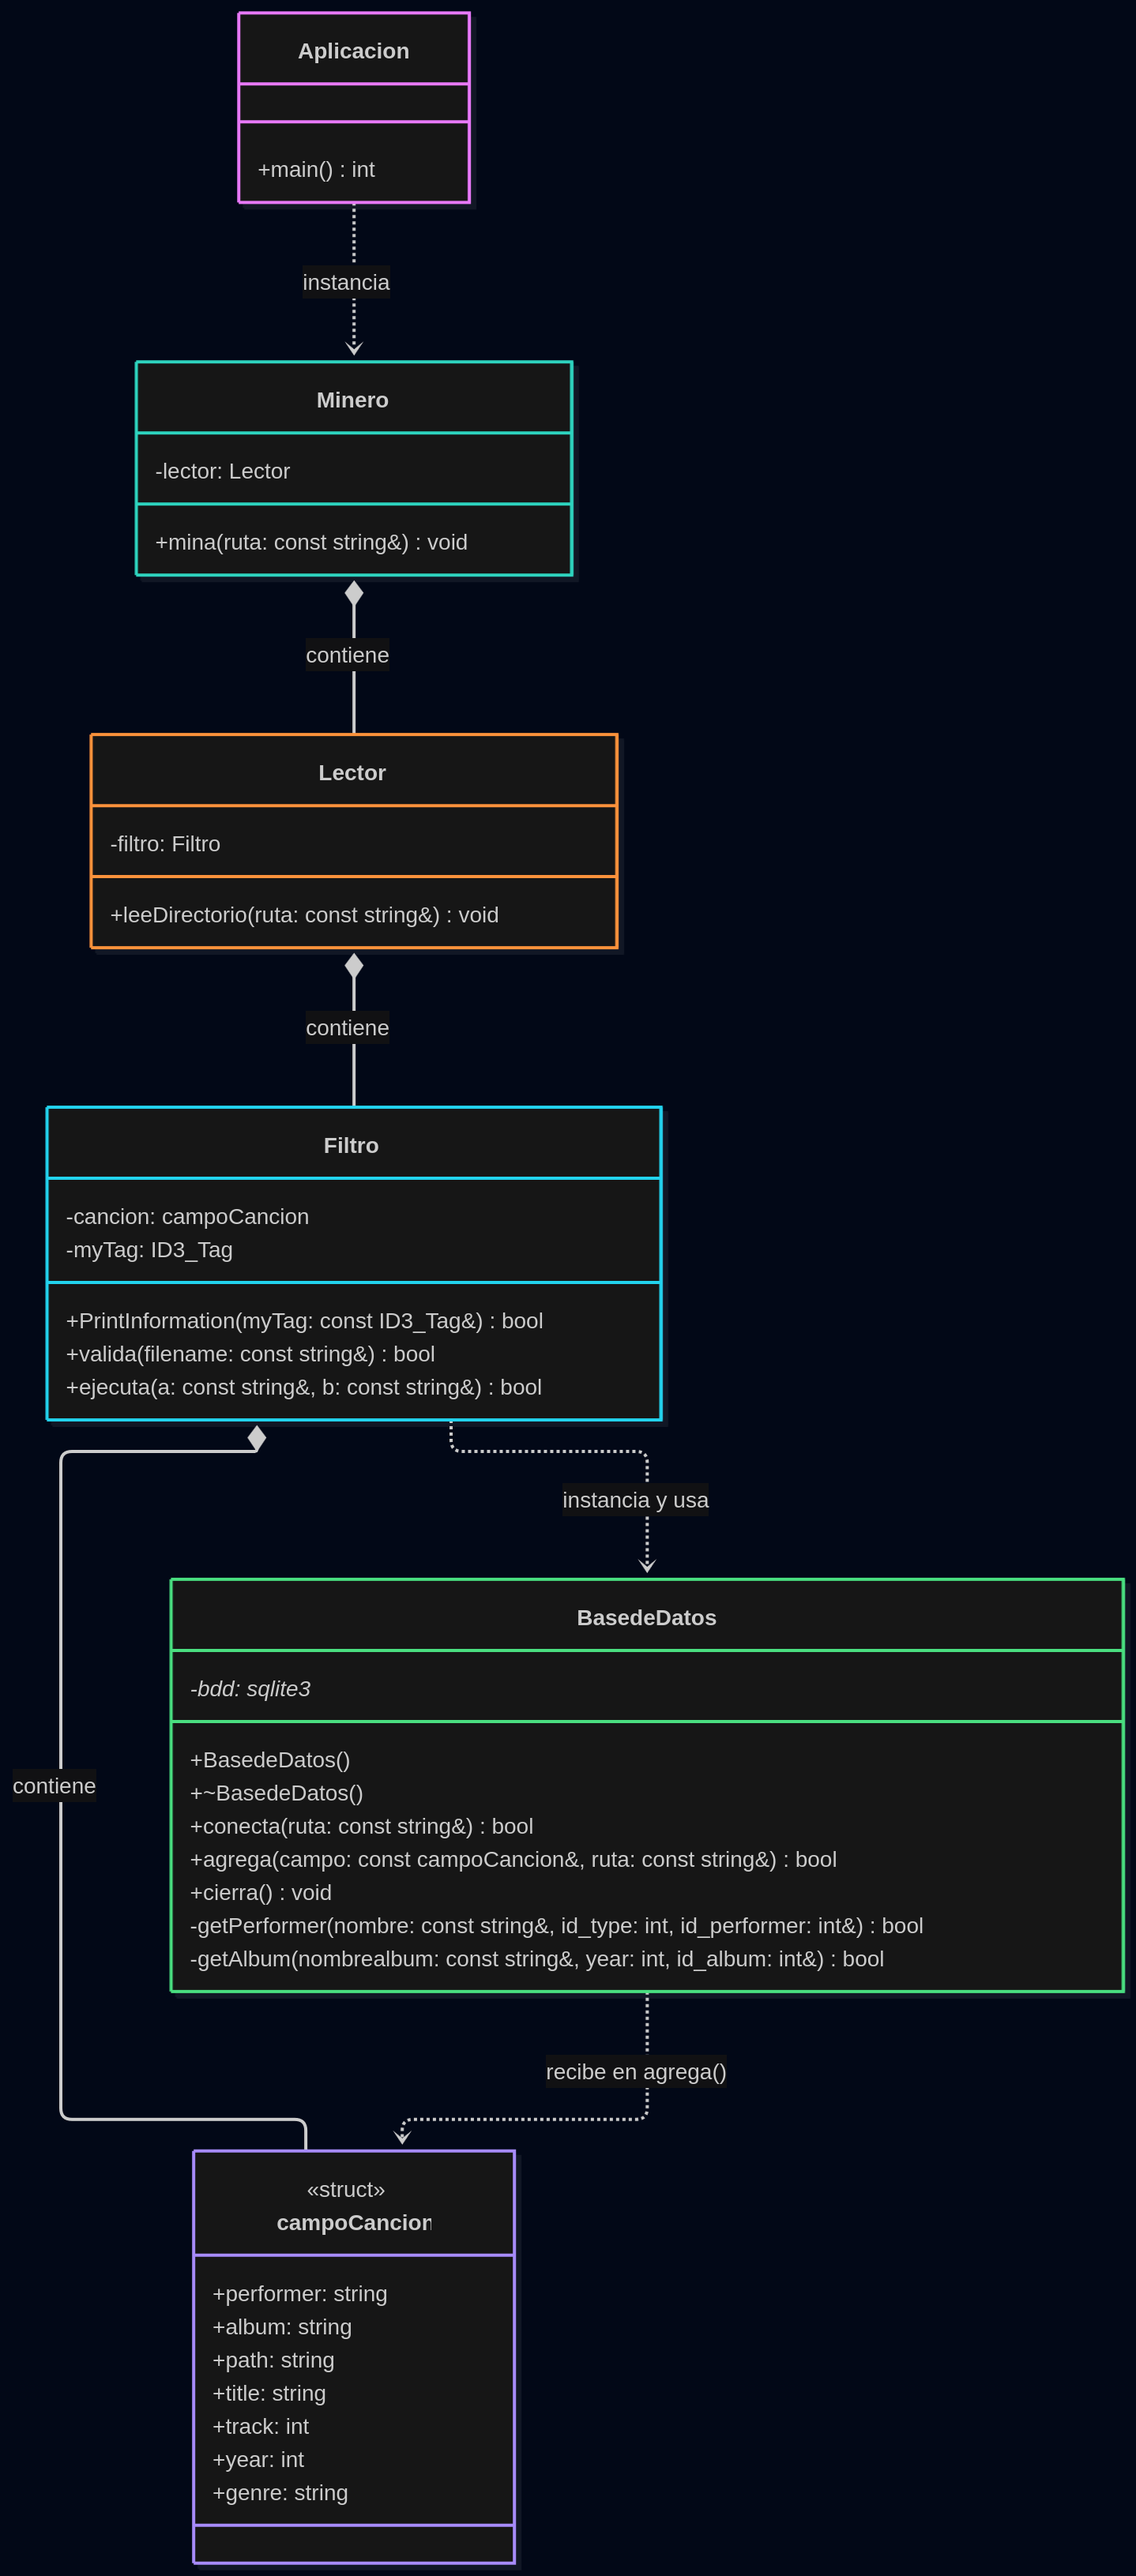
\includegraphics[height=0.80\textheight, keepaspectratio]{images/diagramaMinero.png}
    \caption{Diagrama de clases del minero.}
    \label{fig:diagramaMinero}
\end{figure}

  
  \newpage
  
  \subsection*{Interfaz}
  \subsubsection*{Analisis}
  En la interfaz se deben poder ver las canciones de la base de datos, editarlas y buscar, como es una interfaz gráfica usé el modelo vista controlador, separando así lo que ve el usuario, el controlador y el modelo, en el modelo tengo un programa que ejecuta al minero, una clase que se conecta a la base de datos y un objeto que representa la canción.
  \subsubsection*{Diseño}    
    \subsubsection*{Vista}
    En Views tengo mi ventana, que en un xaml diseño, realmente saqué mucha inspiración de Pinterest así como la imagen de fondo que tiene la tercera columna, la imagen default si no se encuentra la portada y la imagen de mi botón para minar, el diseño de 3 columnas también lo saque de una imagen de pinterest y me ayudé bastante de un tutorial que tenía el framework que escogí de una tienda de música.

    \begin{figure}[htbp]
      \centering
      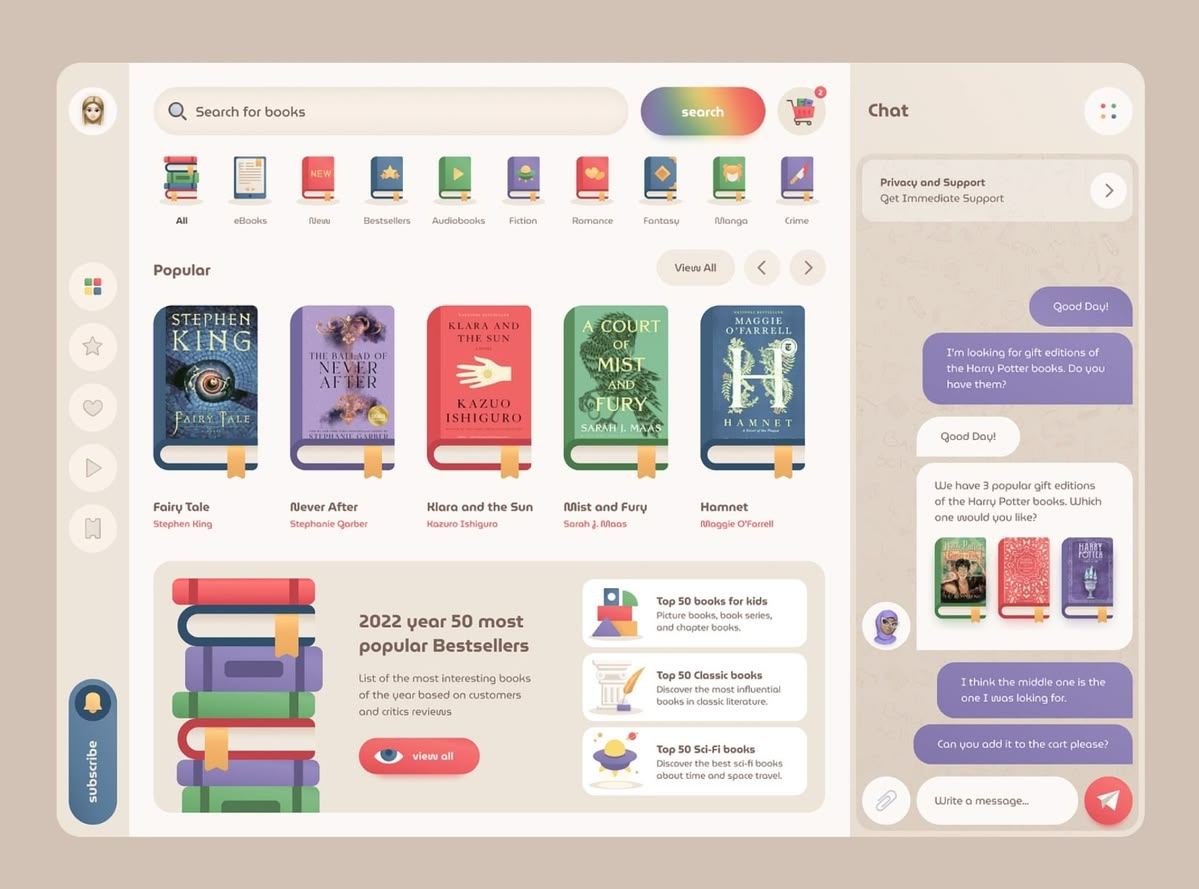
\includegraphics[height=0.40\textheight, keepaspectratio]{images/layoutdepinterest.jpg}
      \caption{Inpiracion de Pinterest}
      \label{fig:Inspo}
    \end{figure}
Cada botón corresponde a una acción en el controlador.

\subsubsection*{Controlador}
Se encuentra en ViewModels/, que primero tiene ModelViewBase.cs que realmente no utlizo, porque la clase importante, MainViewModel.cs hereda de ObservableObject y en esta clase sirve para comunicar la vista y el modelo y con ObservableObject y su propiedad ObservableProperty notifica de los cambios en las propiedades y actualiza automáticamente la vista con los Bindings yRelay Command.
   \newpage   

\subsubsection*{Modelo}
En Models/ tengo 4 clases
 \begin{itemize}
 \item \subsubsection*{Minero}
   en Miner y aplicacionMiner es donde mino, creo que realmente no necesitaba separarlos, pero siento que queda más limpio así, utilizo process para ejecutar el ejecutable de Minero en c++ que cree al instalarlo con meson en ~/.local/share/rolas y es async.
    \item \subsubsection*{bdd}
      Es la conexión con la base de datos y crea las instrucciones para editar y buscar, fue lo que más se me dificultó, e incluso creo que aún tiene ligeros imperfectos.
    \item \subsubsection*{Rola}
      Aqui represento las canciones con los elementos de la tabla rolas como propiedades, lo más complicado fue la portada, como no aparecía en mi ventana la portada con solo la string de la ruta CoverPath, hice un bitmmap para obtenerla, primero ve si el usuario pasó alguna, si no, busca en  ~/.local/share/rolas/imagenes y si no, usa la imagen que tengo como predeterminada y para que no la tenga que cargar cada vez la guarda en un cache, tengo dos métodos auxiliares para esto.
    \item \subsubsection*{Elemento}
     Elemento es para representar registros de la base de datos que no sean de la tabla rolas, solo tiene propiedades.
 \end{itemize}

    
 \newpage
  \begin{figure}[htbp]
      \centering
      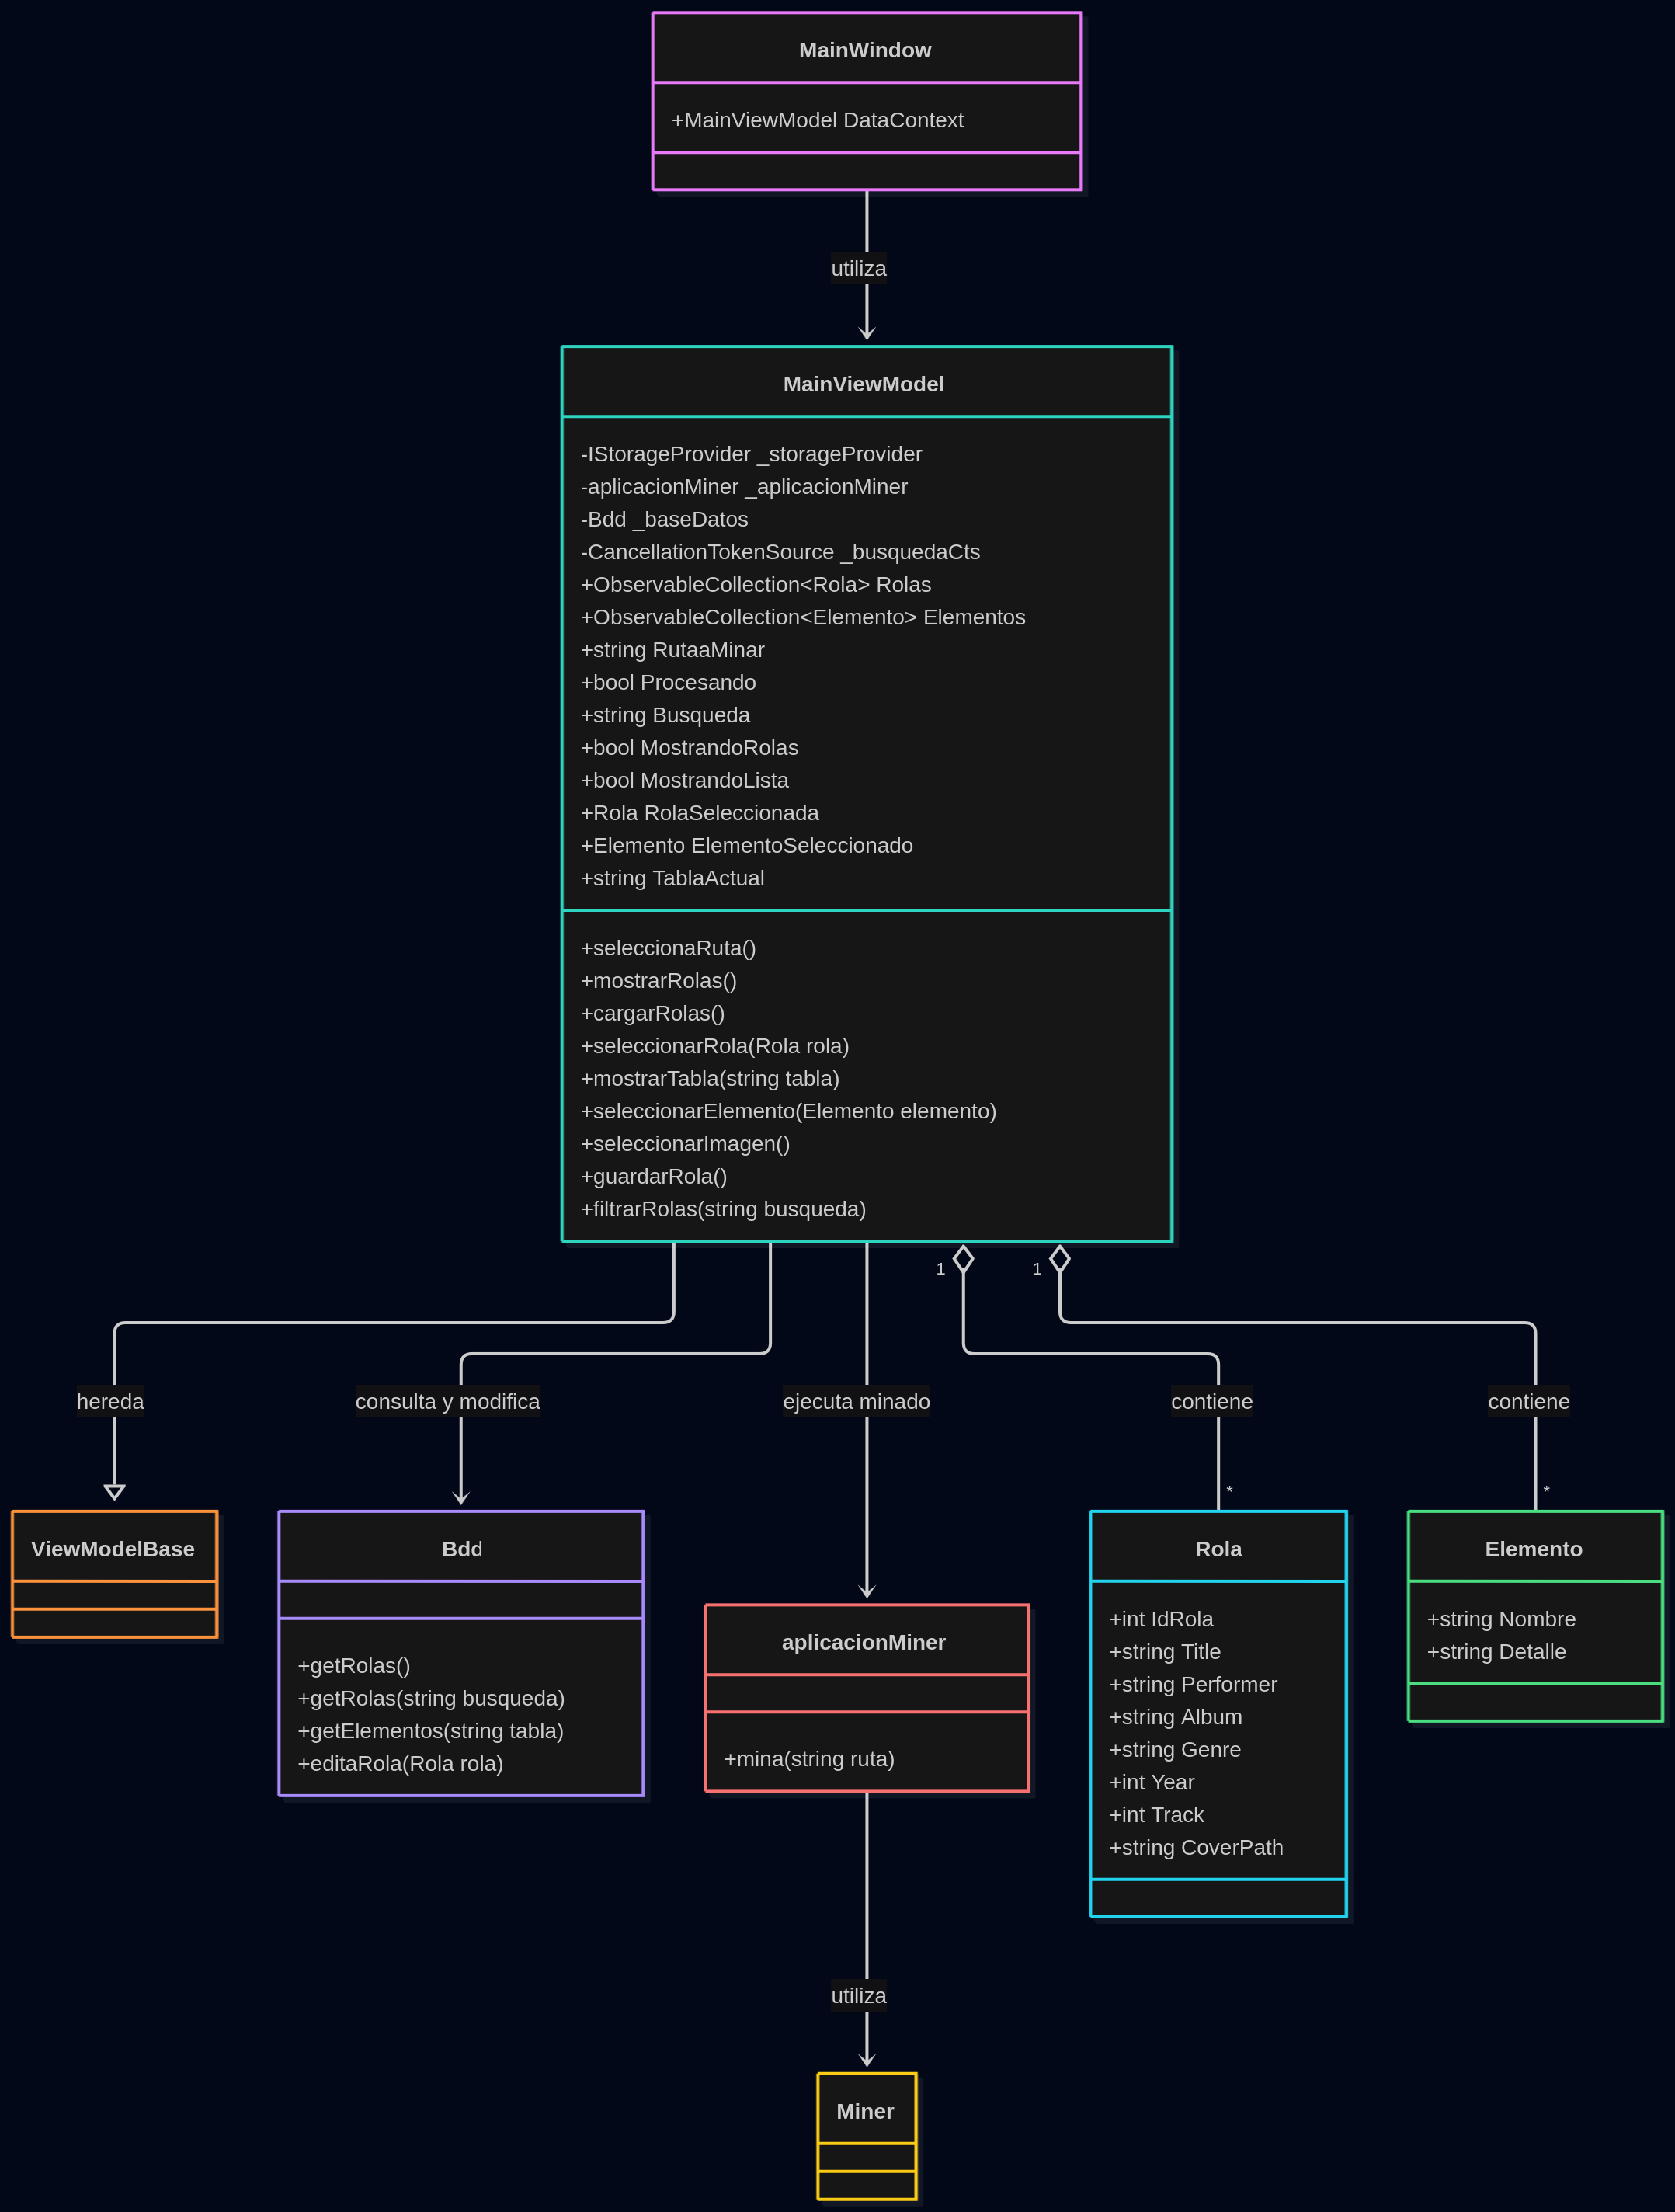
\includegraphics[height=0.80\textheight, keepaspectratio]{images/diagramaInterfaz.png}
      \caption{Diagrama de clase de la interfaz}
      \label{fig:Diagrama}
    \end{figure}
 
 \newpage
  
  \section*{Implementación}
  Para el minero usé el sistema de construccion meson, ya que lo utilicé el proyecto pasado y me gustó, ahí compilo el minero y lo instalo, tambien le paso ciertos parámetros como la dependencia de sqlite3 y la biblioteca de id3 y suprimo una advertencia que tenía al borrar un iterador en Filtro.
  Las bibliotecas que instalé para minero son:
  \begin{itemize}
  \item id3lib 
  \item libsqlite3-dev
  \end{itemize}
  
  Y para la interfaz utilizo el framework de C\# Avalonia, lo escogí porque en su repositorio tienen un tutorial de una tienda de música que se asimila uun poco a lo que hice, tambien porque al crear un proyecto te daba la plantilla para usar el modelo vista controlados y por el binding que hace muy facil conectar la vista y el modelo.
  Necesita al menos .NET 8 e instalar las plantillas, tambien las bibliotecas de sqlite.  
  \newpage
  \section*{Conclusiones}
  Este proyecto me gustó bastante, se me complicó un poco lo de sqlite tanto en el minero como  en la interfaz, también tuve problemas con la interfaz ya que no se estaban mostrando las imagenes de portada, tambíen moví varias cosas de lugar (como donde se instalaba Minero y las imagenes de la base de datos) pero unos compañeros me ayudaron en eso e incluso en como descargar mp3 para probar, pero si es un proyecto que me gusto bastante, incluso me gustó como quedó la interfaa.
  \section*{Resumen}
  Durante este proyecto creé un minero, para recorrer directorios y encontrar archivos y encontrar etiquetas id3 para agregarlos a la base de datos y una interfaz donde puedo usar ese minero, ver las canciones que agregué, buscar de manera muy sencilla entre ellas y editar su información en la base de datos. En este reporte vimos primero una introducción con una descripción del proyecto, luego vimos el proceso de analisis y modelado, hasta llegar a la implementación y luego explicamos las conclusiones.
  
  \newpage
  \section*{Fuentes}
  \begin{itemize}
  \item Ajcvickers. (s.~f.). Información general - Microsoft.Data.Sqlite. Microsoft Learn. \url{https://learn.microsoft.com/es-es/dotnet/standard/data/sqlite/?tabs=net-cli}

    \item Avalonia.Samples/src/Avalonia.Samples/CompleteApps/Avalonia.MusicStore at main $\cdot$ AvaloniaUI/Avalonia.Samples. (s.~f.). GitHub. \url{https://github.com/AvaloniaUI/Avalonia.Samples/tree/main/src/Avalonia.Samples/CompleteApps/Avalonia.MusicStore}

    \item Dmc. (2026, 2 septiembre). Avalonia UI: Introduction and Initial Impression. DMC, Inc. \url{https://www.dmcinfo.com/blog/15658/avalonia-ui-introduction-and-initial-impression/}

    \item Filesystem library (since C++17) - cppreference.com. (s.~f.). \url{https://cppreference-com.translate.goog/cpp/filesystem?_x_tr_sl=en\&_x_tr_tl=es\&_x_tr_hl=es\&_x_tr_pto=tc}

    \item GeeksforGeeks. (2025, 11 julio). SQL using C/C++ and SQLite. GeeksforGeeks. \url{https://www-geeksforgeeks-org.translate.goog/cpp/sql-using-c-c-and-sqlite/?_x_tr_sl=en\&_x_tr_tl=es\&_x_tr_hl=es\&_x_tr_pto=tc\&_x_tr_hist=true}

    \item How to Connect to SQLite from C\# (.NET). (2026, 23 junio). \url{https://mako.ai/guides/sqlite/connect-from-csharp}

    \item id3lib/examples/demo\_info.cpp at master $\cdot$ irwir/id3lib. (s.~f.-a). GitHub. \url{https://github.com/irwir/id3lib/blob/master/examples/demo\_info.cpp}

    \item id3lib/examples/demo\_info.cpp at master $\cdot$ irwir/id3lib. (s.~f.-b). GitHub. \url{https://github.com/irwir/id3lib/blob/master/examples/demo\_info.cpp}

    \item Libreria de colores C / C++. (s.~f.-a). Gist. \url{https://gist.github.com/Alfonzzoj/db207b89d56f24d9d0b17ff93e091be8}

    \item Libreria de colores C / C++. (s.~f.-b). Gist. \url{https://gist.github.com/Alfonzzoj/db207b89d56f24d9d0b17ff93e091be8}

    \item Libreria de colores C / C++. (s.~f.-c). Gist. \url{https://gist.github.com/Alfonzzoj/db207b89d56f24d9d0b17ff93e091be8}

    \item Llamas, L. (2026, 23 julio). What is std::filesystem::path and How to Use It in C++. Luis Llamas. \url{https://www.luisllamas.es/en/cpp-filesystem-path/}

    \item Samples and tutorials | Avalonia Docs. (2026, 9 noviembre). \url{https://docs-avaloniaui-net.translate.goog/docs/samples-tutorials?av_source=marketing\&av_medium=docs_link\&av_content=getting-started\&_x_tr_sl=en\&_x_tr_tl=es\&_x_tr_hl=es\&_x_tr_pto=tc}

    \item TylerMSFT. (s.~f.). path (Clase). Microsoft Learn. \url{https://learn.microsoft.com/es-es/cpp/standard-library/path-class?view=msvc-170}
  \end{itemize}

\end{document}


